\documentclass[11pt]{article}
\usepackage[margin=1in]{geometry}
\usepackage[pdftex]{graphicx}
\usepackage{amsmath,amssymb,amsthm}
\usepackage{custom}
\usepackage{pgfplots}

% color boxes
\usepackage[many]{tcolorbox}
\tcbuselibrary{theorems}
\newtcbtheorem{psexample}{Example}{colback=green!10,colframe=green!40!black,fonttitle=\bfseries,breakable,enhanced}{ex}
\newtcbtheorem{psproblem}{Problem}{colback=blue!10,colframe=blue!40!black,fonttitle=\bfseries,breakable,enhanced}{id}
\newtcbtheorem{psremark}{Remark}{colback=purple!10,colframe=purple!40!black,fonttitle=\bfseries,breakable,enhanced}{rm}
\newtcbtheorem{pssolution}{Solution}{colback=orange!10,colframe=orange!40!black,fonttitle=\bfseries,breakable,enhanced}{sn}
\tcbset{noparskip/.style={before={\par\pagebreak[0]\medskip\parindent=0pt},
after={\par\medskip}}}

% formatting for problems and solutions
\definecolor{ptred}{rgb}{0.7,0.1,0.1}
\newcommand{\ptfmt}[1]{\textbf{\color{ptred}#1\color{black}}}
\definecolor{advblue}{rgb}{0.1,0.1,0.7}
\newcommand{\advanced}{\!\textbf{\color{advblue}[A]\color{black}}\ }

\newtheorem*{solution}{Solution}
\newtheorem*{answer}{Answer}

\makeatletter
\newtheoremstyle{mystyle}
{\topsep}               % space above
{\topsep}               % space below
{}                      % bodyfont
{}                      % indent
{\bfseries}             % headfont
{}                      % punctuation
{0.6em}                 % space after head
{\llap{\hspace{.6em}}\thmname{#1}\thmnumber{ #2}\thmnote{\normalfont{ (#3)}}{\bfseries .}}  %theoremheadspec
\theoremstyle{mystyle}
\newtheorem{pproblem}{Problem}
\makeatother

% headers and footers
\usepackage{fancyhdr}
\pagestyle{fancy}
\lhead{Filip Ramazan}
\chead{}
\rhead{STAT 461}
\lfoot{}
\cfoot{\thepage}
\rfoot{}
\renewcommand{\headrulewidth}{0.4pt}
\setlength{\headheight}{14pt}

\newcommand{\psettitle}[1]{
    \begin{center}
    \huge \textbf{#1}
    \end{center}
}
\newcommand{\x}{\cdot}

\linespread{1.03} % give a little extra room
\setlength{\parindent}{0.2in} % reduce paragraph indent a bit

% uncomment to hide solutions
% \usepackage{environ}
% \NewEnviron{hide}{}
% \let\solution\hide
% \let\endsolution\endhide
% \let\answer\hide
% \let\endanswer\endhide

\begin{document}

\psettitle{Homework \#4}

\noindent

\begin{psproblem}{Dies by Calculation}{}
Suppose a fair die is tossed three times.
\begin{enumerate}[label=\alph*.]
\item Let $X$ be the largest of the faces that appear. Write with justification the probability density function of $X$.
\item Let $Y$ be the number of different faces that appear. Write with justification the probability density function
and the cumulative distribution function $F_Y$ of Y. Plot the graph of $F_Y$ .
\end{enumerate}
\end{psproblem}

\begin{solution}
\leavevmode
\begin{enumerate}[label=\alph*.]
\item Probability mass function of $X$: \[
\begin{array}{c|ccccccc}
    x & 0 & 1 & 2 & 3 & 4 & 5 & 6 \\ \hline
    \rule{0pt}{12pt} % Adds vertical space ONLY to this row without breaking the vertical line
    P(X = x) & \frac{1}{216} & \frac{7}{216} & \frac{19}{216} & \frac{37}{216} & \frac{61}{216} & \frac{91}{216} & \frac{127}{216}
\end{array}
\]
To find the probabilities for each value of $X$, we use the formula $\dfrac{k^3}{6^3}-\dfrac{(k-1)^3}{6^3}$, since $P(x \le k) - P(x \le k-1)=P(x=k)$
\item Probability mass function of $Y$: \[
\begin{array}{c|ccc}
    y & 1 & 2 & 3 \\ \hline
    \rule{0pt}{12pt} % Adds vertical space ONLY to this row without breaking the vertical line
    P(Y = y) & \frac{6}{216} & \frac{90}{216} & \frac{120}{216}
\end{array}
\]
\begin{flalign*}
P(x=1) &= 6 \x 1 \x 1 = 6 \text{, since there must be only 1 distinct number.} &&
P(x=2) &= 6 \x 5 \x 1 = 30 \text{, since there must be 2 distinct numbers, and one repeated.} &&
P(x=3) &= 6 \x 5 \x 4 = 120 \text{, since there must be 3 distinct numbers.} &&
\end{flalign*}
Cumulative distribution function of $Y$:
\[
F_{Y}(t)=
 \begin{cases} 
      0 & t < 1 \\
      \frac{1}{36} & 1 \le t < 2 \\
      \frac{4}{9} & 2 \leq t < 3 \\
      1 & 3 \le t 
   \end{cases}
\]
Plot of $F_Y$:
\begin{center}
\begin{tikzpicture}
    \begin{axis}[
        axis x line=middle, 
        axis y line=middle,
        enlargelimits=true,
        xlabel={$t$},
        ylabel={$F_Y(t)$},
        ymin=-0.1, ymax=1.1,
        xmin=0, xmax=4,
        xtick={1,2,3},
        ytick={0,1/36,4/9,1},
        domain=0:4,
        samples=100,
        width=10cm,
        height=7cm,
        grid=major % Adds major gridlines
    ]
        \addplot[mark=none,blue,thick] coordinates {(-100,0) (1,0)};
        \addplot[only marks,mark=o,blue,thick] coordinates {(2,1/36)}; % Empty circle at discontinuity
        \addplot[only marks,mark=o,blue,thick] coordinates {(1,0)}; % Empty circle at discontinuity
        \addplot[mark=*,fill=white,blue] coordinates {(1,1/36)};
        \addplot[mark=none,blue,thick] coordinates {(1,1/36) (2,1/36)};
        \addplot[mark=*,fill=white,blue] coordinates {(2,4/9)};
        \addplot[only marks,mark=o,blue,thick] coordinates {(3,4/9)}; % Empty circle at discontinuity
        \addplot[mark=none,blue,thick] coordinates {(2,4/9) (3,4/9)};
        \addplot[mark=*,fill=white,blue] coordinates {(3,1)};
        \addplot[mark=none,blue,thick] coordinates {(3,1) (100,1)};
    \end{axis}
\end{tikzpicture}
\end{center}
\end{enumerate}
\end{solution}

\begin{psproblem}{Triple Flip Tally}{}
    A fair coin is flipped three times. Let $Y$ be the number of heads minus the number of tails. Write with justification
    the probability density function and the cumulative distribution function $F_Y$ of $Y$. Plot the graph of $F_Y$.
\end{psproblem}

\begin{solution}
    \leavevmode
    Probability mass function of $Y$: \[
    \begin{array}{c|ccccc}
        y & -3 & -1 & 1 & 3 \\ \hline
        \rule{0pt}{12pt} % Adds vertical space ONLY to this row without breaking the vertical line
        P(Y = y) & \frac{1}{8} & \frac{3}{8} & \frac{3}{8} & \frac{1}{8}
    \end{array}
    \]
    To find the probability for each value of $Y$, we use the formula $\binom{3}{\left| x \right|} \x \dfrac{1}{2^3}$.
    \newline
    Cumulative distribution function of $Y$:
    \[
    F_{Y}(t)=
     \begin{cases} 
          0 & t < -3 \\
          \frac{1}{8} & -3 \le t < -1 \\
          \frac{1}{2} & -1 \le t < 1 \\
          \frac{7}{8} & 1 \le t < 3 \\
          1 & 3 \le t
       \end{cases}
    \]
    Plot of $F_Y$:
    \begin{center}
        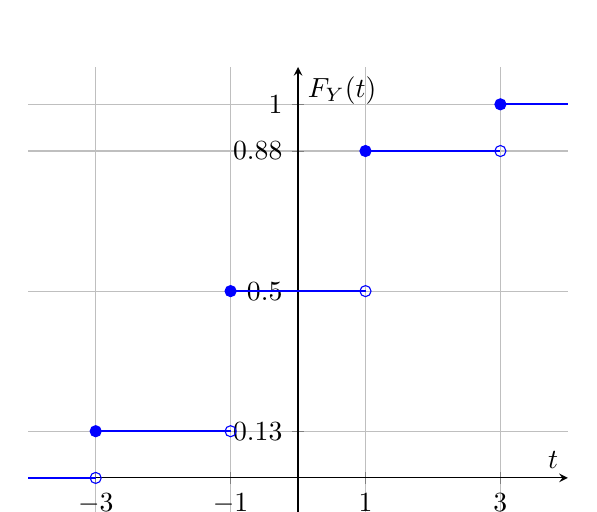
\begin{tikzpicture}
            \begin{axis}[
                axis x line=middle, axis y line=middle,
                xtick={-3,-1,1,3}, ytick={0,1/8,1/2,7/8,1},
                ymin=-0.1, ymax=1.1, xmin=-4, xmax=4,
                xlabel={$t$}, ylabel={$F_Y(t)$},
                domain=-4:4, samples=100, grid=major
            ]
            % Draw step function
            \addplot[blue, thick] coordinates {(-4,0) (-3,0)};
            \addplot[blue, thick] coordinates {(-3,1/8) (-1,1/8)};
            \addplot[blue, thick] coordinates {(-1,1/2) (1,1/2)};
            \addplot[blue, thick] coordinates {(1,7/8) (3,7/8)};
            \addplot[blue, thick] coordinates {(3,1) (4,1)};
        
            % Add open circles for discontinuities
            \addplot[blue, only marks, mark=o] coordinates {(-3,0) (-1,1/8) (1,1/2) (3,7/8)};
            
            % Add filled circles for jumps
            \addplot[blue, only marks, mark=*] coordinates {(-3,1/8) (-1,1/2) (1,7/8) (3,1)};
            \end{axis}
        \end{tikzpicture}
    \end{center}

\end{solution}

\begin{psproblem}{Triple Flip Tally}{}
    Let $X$ be a discrete random variable which can take only the value $x = 0, 1, 2, 3, 4, 5, 6$ such that the cumulative
    distribution function is defined by $F_X(x) = \dfrac{x^2 + x}{42}$ for the above values. Find the probability density function of $X$.
\end{psproblem}
\begin{psproblem}{}{}
    Suppose $X$ is a random variable with binomial distribution $B \displaystyle \left( 4, \dfrac{2}{3} \displaystyle \right)$. Find the probability density function of
    $2X + 1$.
\end{psproblem}
\begin{psproblem}{}{}
    Suppose that only $30\%$ of all drivers come to a complete stop at an intersection. Let $X$ be the number of drivers
    which come to a complete stop, among $10$ randomly chosen drivers coming to an intersection.
    \begin{enumerate}[label=\alph*.]
        \item What is the probability distribution of $X$?
        \item Determine $P(X = 2)$.
        \item Determine the probability that at least $2$ out of the $10$ drivers will come to a complete stop.
        \item What is the most likely number of drivers to come to a full stop among $10$ drivers?
    \end{enumerate}
\end{psproblem}
\begin{psproblem}{}{}
    Of the items manufactured by a certain process, $20\%$ are defective. Of the defective items $60\%$ can be repaired.
    \begin{enumerate}[label=\alph*.]
        \item Find the probability that a randomly chosen item is defective and cannot be repaired.
        \item Find the probability that exactly $2$ of $20$ randomly chosen items are defective and cannot be repaired.
    \end{enumerate}
\end{psproblem}
\begin{psproblem}{}{}
    A distributor receives a large shipment of components. The distributor would like to accept the shipment if 10
    or fewer of the components are defective and to return it otherwise. She decides to sample 10 components and to
    return the shipment if more than 1 component is defective.
    \begin{enumerate}[label=\alph*.]
        \item If the proportion of defectives in the batch is in fact 10\%, what is the probability that she will return the
        shipment?
        \item If the proportion of defectives in the batch is in fact 20\%, what is the probability that she will return the
        shipment?
        \item The distributor decides to accept the shipment only if none of the components in the batch is defective. What
        is the minimum number of items she should sample if she wants a probability no greater than 1\% of accepting
        the shipment if 20\% of the items are defective?
    \end{enumerate}
\end{psproblem}





%\begin{psexample}{Example Title}{}
%Example
%\end{psexample}
%
%\begin{pssolution*}{}{}
%Solution
%\end{pssolution*}
%
%\begin{psremark*}{Remark Title}{}
%Remark
%\end{psremark*}
%\begin{pproblem} \clock{0}{30}
%Problem statement
%\end{pproblem}

\end{document}